\chapter{Java and memory}
\label{chap:javamem}

As previously noted, the way programming languages model memory is very
different from how it is implemented in hardware. This is especially true for
high-level languages, and doubly so for managed platforms like Java.

Java programmers cannot directly control things like memory barriers and memory
layout. Instead we get the effect of barriers through judicious use of the
\java{synchronized} and \java{volatile} keywords, the classes in the
\\\java{java.util.concurrent} package, and the guarantees given by
the Java Language Specification\cite{javaspec}.
The language specification gives no such guarantees regarding memory
layout, making it is harder to control: We can take steps to affect how
data is laid out in memory, and we can verify the effectiveness of our efforts
by benchmarking our programs, but we do not have guarantees that our
optimizations will work on other Java runtimes, or with future Java versions.

In the following sections we first look at the relationship between Java's
concurrency constructs and the memory hardware as described in chapter
\ref{chap:arch}, then we look at 7 techniques for manipulating the memory layout
in Java.

\section{Data sharing}
In Java, the concept of \textit{happens-before order} most closely captures the
purpose of memory barriers, in that it guarantees that memory operations are
visible to relevant threads/CPU-cores, and that they appear to happen in the
expected order.

The way we interact with the cache coherence protocol in the Java memory model
does not correspond directly to the hardware view we have from
\cite{mckenny-barriers}: From this hardware oriented point of view, memory
barriers are invoked specifically to flush store buffers and invalidation
queues, ensuring coherence with all other cores that do or have done the same.
In Java, happens-before order is not something we ensure with an instruction or
method, rather it is guaranteed when we interact in certain ways with
synchronization variables like locks and \java{volatile} fields. One could say
that in Java visibility is something we "get" rather than something we "do".
This high-level and non-imperative style of incorporating multicore coherence
into an object-oriented language is rather elegant, but it makes it easy to
overlook concurrency constructs in code: Removing code that causes a seemingly
unnecessary read can have important consequences if the read was to a
\java{volatile} field. It also forces software designers to use strange looking
constructs, such as wrapping primitive types in seemingly useless wrapper
classes, just so their fields can be declared \java{volatile}.

\begin{code}
\begin{Verbatim}[frame=single]
  public static class Holder {
    public volatile int value;
  }
\end{Verbatim}
	\caption{}
	\label{code:holder}
\end{code}

Java provides no mechanism for guaranteeing visibility of updates to array
elements. Declaring the array \java{volatile} will only affect the array field
itself, not its contents. An array of instances of the \java{Holder} class in
code snippet \ref{code:holder} can be used to effectively make an array of
volatile elements: Instead of replacing the elements of the array, we confine
ourselves to updating the \java{volatile} \java{value} fields of the
\java{Holder} objects. Of course, we still need to ensure that that the
initialization of the array elements is made visible. The downside of this
technique, besides the silly wrapper class, is that it requires more memory.
Each \java{Holder} instance takes up 16 bytes of memory instead of the 4 bytes
an \java{int} would have used (we will see evidence for these numbers in the
next section).
There is also the additional memory overhead of storing the object pointers in
the array. Additionally, there is the performance cost of the added indirect, as
accessing the elements now requires reading the object pointer from the array,
and \textit{then} reading the object.

The implementers of the Java Class Library seem to favour the undocumented
\java{sun.misc.Unsafe} class for this kind of synchronization difficulty. With
regard to whether the \java{Unsafe} class should be used, I will
let the name of the class and the fact that it is an unpublished, undocumented part
of the api speak for itself. For readers who are undeterred by such details,
Doug Lea's implementations of the \java{AtomicInteger} \cite{atomicintegersrc},
\java{AtomicIntegerArray} \cite{atomicinterarraysrc},
\java{LongAdder} \cite{longaddersrc}, and \java{Striped64} \cite{striped64src}
classes are well commented, highly illustrative, and well suited for learning
about both the \java{Unsafe} class and multicore software design in
general.

To facilitate mutual exclusion, Java provides locking mechanisms through the
\java{synchronized} keyword, and through the \\
\java{java.util.concurrent.locks}
package. Lock implementations vary with the underlying hardware, and are usually
provided by the operating system. The details therefore depend on the runtime
platform, but the use of memory barriers and compare-and-swap appears to be
ubiquitous. This means lock operations depend on the cache coherence protocol,
which makes them subject to false sharing overhead. It is not immediately
obvious that the actual lock data is stored in the object headers on the heap:
The Java virtual machine could in theory keep a global table of locks. In
\cite{mystery} \citeauthor{mystery} found that spacing the allocation of locks
significantly improves performance in a multicore context, leading us to believe
that lock data is indeed stored in the object headers of the lock object. This
means we can prevent false sharing of locks if we can avoid dense allocation of
locks on the heap.

Like the mechanisms provided to us, the guarantees provided by the Java memory
model do not correspond directly to those we know from hardware. Reading
from a \java{volatile} field ensures the visibility of updates made by other
threads \textit{before they wrote to the same field}. With what we know from
\cite{mckenny-barriers}, it is not clear why threads reading a
\textit{different}
\java{volatile} field do not get the same guarantee.

The remainder of this report will nonetheless show that the hardware view taken
in \cite{mckenny-barriers} is very useful when considering the multicore
performance of Java programs. For this reason, with respect to multicore performance, we adopt
the view that whenever the Java memory model guarantees happens-before-order, it
does so through the use of memory barriers. This implies that e.g. accessing
\java{volatile} fields, or taking or releasing a lock, causes the CPUs
invalidation queues and store buffers to be flushed. Hence the cost of the
coherence protocol is vastly increased for operations that guarantee
happens-before-order.

\section{Memory layout} Almost no promises are made regarding memory layout in
Java. It appears to be true that objects as well as arrays are stored as
contiguous memory segments,
but this is entirely at the discretion of the implementers of the Java virtual
machine in use. It seems that the only guarantees are that instance
fields, static fields, and array \textit{elements} are stored on the heap, and
that local variables, formal method parameters, and exception handler parameters
are not\cite[chapter~17]{javaspec}\cite[chapter~2]{jvmspec}. The Java memory
model is only concerned with data allocated on the heap, as stack memory is not
shared between threads. In fact, the Java Virtual Machine
Specification\cite{jvmspec} says very little about how the heap must be defined,
except that it is shared between threads.

\subsection{Padding techniques}
The lack of guarantees regarding memory layout does not mean that all hope is
lost. In the remainder of this chapter we look at ways to manipulate the Java
runtime into adapting the memory layout we want. We will do so armed only with
educated guesswork about how arrays and objects are allocated on the heap, and
the OpenJDK's JOL tool (Java Object Layout).

The JOL tool can be found at
\url{http://openjdk.java.net/projects/code-tools/jol/}

\subsubsection{Spacing array elements}

Let us first consider an array of primitive integers:

\begin{code}[h]
\begin{Verbatim}[frame=single]
  int[] arr = new int[n];
\end{Verbatim}
	\caption{}
\end{code}

While it is not guaranteed, it is reasonable to assume that the elements of such
an array will be stored in a contiguous memory segment on the heap. Indeed,
experiments with locks in \cite{mystery}, as well as our own experiments in
chapter \ref{chap:experiments}, seem to confirm this assumption. This means
array elements of primitive types are prime candidates for false sharing:
Java \java{int}s are 4 bytes, so there will be $64/4 = 16$ elements per
64-byte cache line. If different array elements inside the same cache line are
accessed by different threads, we get false sharing overhead as described in
chapter \ref{chap:arch}. For such use cases, it makes sense to spread the
elements out in memory, by leaving unused "padding" between them. We will refer
to this as a "spaced" or "padded" layout, as opposed to the normal "dense"
layout.

\begin{padding}[h]
\begin{Verbatim}[frame=single]
  //allocation
  int[] arr = new int[n + n * p];
  //access
  int i = ...; // index if no padding were used
  arr[i + (i+1) * p] = ...;
\end{Verbatim}
	\caption{Spaced allocation of array elements of a primitive type}
	\label{padding:primitive-array}
\end{padding}

Padding technique \ref{padding:primitive-array} allows us to introduce padding
in arrays of primitive types.
To have $n$ useful array elements, each with $p$ padding elements before it, we
declare an array of length $n + n * p$. We then find the $i$'th useful element
at index $i + (i+1) * p$. We elect to add padding before, rather than after,
each element under the assumption that there is shared information, such as
the array length, stored immediately \textit{before} the first array element.
This may not actually be the case.

\subsubsection{Padding between objects}
Arrays of object types are a little more complicated.
If we wish to prevent objects in an array from sharing cache lines -- e.g.
when using a \java{volatile} wrapper like the \java{Holder} class -- padding technique
\ref{padding:primitive-array} is insufficient. Unlike arrays of primitive
types, it appears that arrays of object types do not contain the actual objects.
Rather, they store an object pointer for each array element, pointing to the
actual object on the heap. This behaviour is not specified in the standards, but
it is a sensible implementation: Objects of the same supertype may not use the
same amount of heap space. Computing the address of an array element from the
base pointer and index would therefore be impractical, were the objects
stored directly in the array.

To achieve a spaced memory layout with arrays of object types, we must pad the
\textit{object allocation} itself.

\begin{padding}[h]
\begin{Verbatim}[frame=single]
  Holder[] arr = new Holder[n + n * pa]
  for (int i = 0; i < n; i++) {
    //padding allocation
    for(int j=0; j <= pb; j++){
      int[] dummy = new int[1];
    }
    //useful allocation
    arr[i + (i+1) * pa] = ...;
  }
\end{Verbatim}
	\caption{Spaced allocation of an object type on the heap, and of the
	array elements pointing to the instances.}
	\label{padding:object-array}
\end{padding}

\begin{figure}
	\fbox{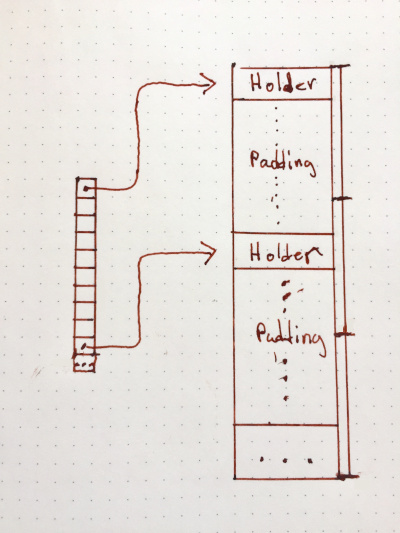
\includegraphics[width=1\textwidth]{img/padding.jpg}}
	\caption{The memory layout achieved with padding technique
	\ref{padding:object-array}. Each dotted row is 8 bytes. To the left we
	see the array of object pointers, with 64 unused bytes between two
	pointers. To the right we see the \java{Holder} instances on the heap.
	Each instance occupies 16 bytes of space, followed by 64 bytes of unused
	\java{int} arrays. The markings on the right side indicate cache line
	boundaries. The division between the array on the left and the objects
	on the right is stylistic: They are both allocated on the heap.}
	\label{fig:spacedholders}
\end{figure}

Padding technique \ref{padding:object-array} lets us allocate object
types with padding between them. In addition to the objects, an array of
pointers to the objects is allocated using the idea from technique
\ref{padding:primitive-array}. The variables \texttt{pa} and \texttt{pb}
represent the number of unused array elements we want before each useful
element, and the number of times we wish to run the allocation loop,
respectively. Assuming that an object pointer is 4 bytes long and a singleton
\java{int} array is 8 bytes (the \java{int} itself plus an int \java{int} to
store the array length), $64/4 = 16$ and $64/8 = 8$ are good values for
\texttt{pa} and \texttt{pb} when cache lines are 64 bytes. We may need to keep
references to the dummy arrays somewhere. Otherwise the garbage collector may
remove them and compact the objects into the space occupied by the arrays.
Figure \ref{fig:spacedholders} depicts the memory layout achieved with technique
\ref{padding:object-array}. The figure makes it clear that we are using more
padding than necessary, causing the \java{Holder} instances to shift around in
the cache lines. We could fix this by subtracting the size of a \java{Holder}
from the amount of padding we use, but it would make it harder to write
generalised methods for padding. The same applies to spacing the elements in the
array.

Padding both the object allocation and the array elements means we can update
both array elements and object fields without risk of false sharing. In the
code, we use \java{int}  arrays as padding on the heap. We can use anything, but it is
prudent to use something with a known size. To this end arrays or plain
\java{Object} instances are useful; as we can make slightly less uneducated
guesses about their sizes, than we can for arbitrary object types.

\subsubsection{Array indexing with indirects}

\begin{padding}[h]
\begin{Verbatim}[frame=single]
  public static Pair<int[],int[]> paddingIndirect(
                                    int n, int p) {
    int[] arr = new int[n + n * p];
    int[] indirect = new int[n];
    for(int i = 0; i < n; ++i) {
      indirect[i] = i + (i + 1) * p;
    }
    return new Pair<int[],int[]>(indirect, arr);
  }
\end{Verbatim}
	\caption{Defining an array of indirected indices to facilitate spaced
	allocation of array elements of primitive types}
	\label{padding:primitive-array-indirect}
\end{padding}

Padding technique \ref{padding:primitive-array-indirect} gives us a different way to
work with padded arrays. It works the same way as padding technique
\ref{padding:primitive-array}, but instead of computing the indices of
useful elements each time we need them, we store them in an indirection array.
This simplifies code using the padded array, as the $i$'th
useful element is now accessed as \verb|arr[indirect[i]]|. This technique has the
disadvantage of needing extra memory to store the indirection array. Array
accesses may also get considerably slower, as the extra memory read is likely
much more expensive than computing the index was. Depending on the access
pattern, the cost of the extra memory read may be hidden by cache prefetch
mechanisms.

In addition to the better readability, I prefer this padding technique for many
of our experiments because it might introduce less noise. Certain amounts of
padding, such as 0 or a power of two, could be optimized by the compiler or
hardware. The cost of the extra memory access is less likely to vary with the
amount of padding.

In the same way we expanded padding technique \ref{padding:primitive-array} to
work for object types, which lead us to technique \ref{padding:object-array}, we
can expand technique \ref{padding:primitive-array-indirect} to work with object
types by spacing the object allocation on the heap.
\refstepcounter{padding}\label{padding:object-array-indirect}
To avoid repetition, we will skip the code for this, and simply refer to it at
as padding technique \ref{padding:object-array-indirect}.

\subsubsection{Padding within objects}

Instead of having padding between objects, we can write classes that include
padding inside the object instances. This has two advantages: Having the
padding inside the instances is more resistant to compaction by the garbage
collector, as the padding will be moved along with the object instance. It also
makes code using the objects clearer by abstracting the use of padding into the
class definition. On the other hand, we may still need to pad data structures
used to contain the instances, and having unused fields in class definitions
will not necessarily be clearer than using padding when allocating the
instances.

To leverage object field layout for padding, we need to understand how
objects are laid out in memory. To this end, we rely on the aforementioned
JOL tool. It is tempting to simply disassemble the class files with
javap, but
the runtime's class loader is free to reorder object fields, so the class files
tell us very little about memory layout. JOL works by instantiating classes and
analysing them at runtime, allowing us to see how they are actually laid out.

Running JOL's internals command against \java{java.lang.Object} gives the
output shown in figure \ref{jol:object}.

\begin{figure}
\begin{Verbatim}[frame=single, numbers=left]
# Running 64-bit HotSpot VM.
# Using compressed oop with 0-bit shift.
# Using compressed klass with 3-bit shift.
# Objects are 8 bytes aligned.
# Field sizes by type: 4, 1, 1, 2, 2, 4, 4, 8, 8 [bytes]
# Array element sizes: 4, 1, 1, 2, 2, 4, 4, 8, 8 [bytes]

Instantiated the sample instance via default constructor.

java.lang.Object object internals:
 OFFSET  SIZE   TYPE DESCRIPTION
      0     4        (object header)
      4     4        (object header)
      8     4        (object header)
     12     4        (loss due to the next object
alignment)
Instance size: 16 bytes
Space losses: 0 bytes internal + 4 bytes external = 4
bytes total
\end{Verbatim}
	\caption{}
	\label{jol:object}
\end{figure}

An additional VALUE column has been omitted to save space.

There is a lot of useful information in the output. Let us dissect some of it
before we move on to padding the objects.
The first line tells us that we are running the HotSpot JVM on a 64-bit machine.
The second line tells us that ordinary object pointers (oop) are compressed,
with 0-bit shift. Compression and shifting are techniques used by the JVM to
save space. The details of these techniques are not pertinent to our work, so we will suffice
it to say that object pointers are compressed, which in our case means they are 4 bytes long (we will see this later).
The fourth line tells us that objects are 8 byte aligned. This means that
objects are stored at memory locations that are multiples of 8 bytes, hence any
objects size is effectively a multiple of 8 bytes. If they are not, unused
bytes will be left between objects to achieve 8 byte alignment. Lines 11-16 show
the layout of the object fields, and lines 17-19 summarize the object's memory
footprint. We can see from the output that an \java{Object} instance takes up 16
bytes on the heap, of which 12 are the object headers, and 4 are padding added
so that the next item on the heap will be 8 byte aligned. This is why instances
of the \java{Holder} class from earlier do not need more space than
\java{Object} instances: The \java{int} field fills out the 4 bytes used for 8 byte
alignment for \java{Object}.

Now that we have familiarized ourselves with JOL's output, let us take a look at
the \java{NormalCluster} class -- our version of the unpadded \java{Cluster}
class from \cite{mystery}.

\begin{code}
\begin{Verbatim}[frame=single]
  public static class NormalCluster implements Cluster {
    private volatile Point mean;
    private double sumx, sumy;
    private int count;
    ...
  }
\end{Verbatim}
	\caption{The fields of the \java{NormalCluster} class}
	\label{code:normalcluster}
\end{code}

\begin{figure}[h]
\begin{Verbatim}[frame=single, numbers=left]
com.kmeans.Clusters$NormalCluster object internals:
 OFFSET  SIZE               TYPE DESCRIPTION
      0     4                    (object header)
      4     4                    (object header)
      8     4                    (object header)
     12     4                int NormalCluster.count
     16     8             double NormalCluster.sumx
     24     8             double NormalCluster.sumy
     32     4   com.kmeans.Point NormalCluster.mean
     36     4                    (loss due to the next
object alignment)
Instance size: 40 bytes
Space losses: 0 bytes internal + 4 bytes external = 4
bytes total
\end{Verbatim}
	\caption{JOL output for the unpadded \java{NormalCluster} class}
	\label{jol:normalcluster}
\end{figure}

Code snippet \ref{code:normalcluster} shows the field declarations of the
\java{NormalCluster} class. All of our cluster implementations contain these
fields. They only differ by how many unused padding fields they contain.

As is made clear in \cite{mystery}, and as will be reiterated in chapter
\ref{chap:experiments}, we want to make sure that different \java{Cluster}
instances do not share cache lines. Furthermore, we would
ideally like to have the \java{count}, \java{sumx}, and \java{sumy} fields
together in a single cache line, and the \java{mean} field in it's own
cache line, separate from the other fields.

The output from JOL, shown in figure \ref{jol:normalcluster}, shows us that all four fields are stored in a contiguous
memory section of 28 bytes, followed by 4 bytes for alignment. Accounting for 8 byte alignment and object headers
this means that, in the worst case, we can have all the fields of one
\java{Cluster} instance plus the \java{count}, \java{sumx}, and \java{sumy}
fields of another instance in the same 64-byte cache line.

It seems that Java runtimes in general follow the same strategy for laying out
object fields. Assuming 8 byte alignment: Fields are arranged in descending
order of size. The sort appears to be stable, so the field order in the source code
matters to some extent. If the field segment is not 8 byte aligned -- due to the size of the object
headers not being a multiple of 8 bytes -- a 4 byte field is moved ahead of the
other fields if one exists. That way, the rest of the fields are 8 byte aligned.
We see this in the JOL output for the \java{NormalCluster} class, where
\java{count} is moved to before the \java{sumx} field.

We can abuse this knowledge not only to pad objects, but to pad between fields
as well.

\begin{padding}[h]
\begin{Verbatim}[frame=single]
  public static class PaddedCluster implements Cluster {
    private volatile Point mean;
    private int dummy1, dummy2, dummy3, dummy4, dummy5,
                dummy6, dummy7, dummy8, dummy9, dummy10,
                dummy11, dummy12, dummy13, dummy14
                dummy15, dummy16, dummy17;
    private double dDummy1, dDummy2, dDummy3, dDummy4,
                   dDummy5, dDummy6, dDummy7, dDummy8;
    private double sumx, sumy;
    private long count;
    ...
  }
\end{Verbatim}
	\caption{Manipulating object field layout with unused fields.}
	\label{padding:object-fields}
\end{padding}

\begin{figure}[h]
\begin{Verbatim}[frame=single, numbers=left]
com.kmeans.Clusters$PaddedCluster object internals:
 OFFSET  SIZE               TYPE DESCRIPTION
      0     4                    (object header)
      4     4                    (object header)
      8     4                    (object header)
     12     4                int PaddedCluster.dummy1
     16     8             double PaddedCluster.dDummy1
     24     8             double PaddedCluster.dDummy2
     32     8             double PaddedCluster.dDummy3
     40     8             double PaddedCluster.dDummy4
     48     8             double PaddedCluster.dDummy5
     56     8             double PaddedCluster.dDummy6
     64     8             double PaddedCluster.dDummy7
     72     8             double PaddedCluster.dDummy8
     80     8             double PaddedCluster.sumx
     88     8             double PaddedCluster.sumy
     96     8               long PaddedCluster.count
    104     4                int PaddedCluster.dummy2
    108     4                int PaddedCluster.dummy3
    112     4                int PaddedCluster.dummy4
    116     4                int PaddedCluster.dummy5
    120     4                int PaddedCluster.dummy6
    124     4                int PaddedCluster.dummy7
    128     4                int PaddedCluster.dummy8
    132     4                int PaddedCluster.dummy9
    136     4                int PaddedCluster.dummy10
    140     4                int PaddedCluster.dummy11
    144     4                int PaddedCluster.dummy12
    148     4                int PaddedCluster.dummy13
    152     4                int PaddedCluster.dummy14
    156     4                int PaddedCluster.dummy15
    160     4                int PaddedCluster.dummy16
    164     4                int PaddedCluster.dummy17
    168     4   com.kmeans.Point PaddedCluster.mean
    172     4                    (loss due to the next
object alignment)
Instance size: 176 bytes
Space losses: 0 bytes internal + 4 bytes external = 4
bytes total
\end{Verbatim}
	\caption{JOL output for padding technique \ref{padding:object-fields}}
	\label{jol:paddedcluster}
\end{figure}

Padding strategy \ref{padding:object-fields} lets us accheive the desired
layout of the \java{Cluster}s. The jol output for this implementation can be
seen in figure \ref{jol:paddedcluster}. We add 8 8-byte \java{double}s to clear
out a cache line before the fields, 16 4-byte \java{int}s to separate the
\java{mean} field from the others, and an additional 4-byte \java{int} because
one of them gets moved up to improve alignment.

\subsubsection{Padding with inheritance}

\begin{padding}[h]
\begin{Verbatim}[frame=single]
  public class PaddedRegions
    ...
    public class RegionA {
      protected int a;
      protected int b;
    }
    ...
    public class RegionB {
      protected int c;
    }
    ...
  }
\end{Verbatim}
	\caption{}
	\label{padding:object-inheritance}
\end{padding}

It appears that superclass fields are not in-lined in subclass instances.
Padding technique \ref{padding:object-inheritance} exploits this in order to
segment regions of fields into different cache lines. The technique can be
combined with technique \ref{padding:object-array} or
\ref{padding:object-fields} to gain more fine-grained control of the amount of
padding used. The JOL output can be seen in figure \ref{jol:object-inheritance}

Used with inner-classes, this can be an expressive technique for segmenting
fields in to separate memory regions with clear syntactical boundaries. This may
result in code that is more readable than when using technique
\ref{padding:object-fields} by itself.

\begin{figure}[h]
\begin{Verbatim}[frame=single, numbers=left]
RegionA object internals:
 OFFSET  SIZE            TYPE DESCRIPTION
      0     4                 (object header)
      4     4                 (object header)
      8     4                 (object header)
     12     4             int RegionA.a
     16     4             int RegionA.b
     20     4   PaddedRegions RegionA.this$0
Instance size: 24 bytes
Space losses: 0 bytes internal + 0 bytes external = 0
bytes total

...

RegionB object internals:
 OFFSET  SIZE            TYPE DESCRIPTION
      0     4                 (object header)
      4     4                 (object header)
      8     4                 (object header)
     12     4             int RegionB.c
     16     4   PaddedRegions RegionB.this$0
     20     4         (loss due to the next object
alignment)
Instance size: 24 bytes
Space losses: 0 bytes internal + 4 bytes external = 4
bytes total
\end{Verbatim}
	\caption{Output from running JOL against each of the classes in padding
	technique \ref{padding:object-inheritance}}
	\label{jol:object-inheritance}
\end{figure}

\subsubsection{The Contended annotation}

\begin{padding}[h]
\begin{Verbatim}[frame=single]
  public static class PaddedClusterContended implements
    Cluster {
    @Contended("group1")
    private volatile Point mean;
    @Contended("group2")
    private double sumx, sumy;
    @Contended("group2")
    private long count;
    ...
  }
\end{Verbatim}
	\caption{}
	\label{padding:contended}
\end{padding}

Finally, padding technique \ref{padding:contended} uses an undocumented
annotation\\
\java{sun.misc.Contended} for this exact purpose. It is undocumented,
so there is no guarantee it will work on any particular Java runtime, or that it
won't be removed in the future. However, this is true for all the padding
techniques we have examined. Using the \java{@Contended} annotation yields a
compiler warning: "warning: Contended is internal proprietary API and may be
removed in a future release". It is not clear if using the annotation affects
licensing.

A clear disadvantage of this technique is that we have no control over the
amount of padding used. Advantages of this technique is that the runtime
platform can clearly see that we intend to use padding, and may prevent the
garbage collector from compacting our memory layout.

JOL's internals command does not show any results of using the \java{@Contended}
annotation, but the output of the estimates command can be seen in figure
\ref{jol:contended}. We can see that several large (128-132) unused memory
regions have been added to the instance. The annotation takes an optional
argument for the name of the field group. Fields annotated using the same
argument are put in a contiguous memory segment. The \java{@Contended}
annotation can also be used on class declarations.

\begin{figure}[h]
\begin{Verbatim}[frame=single, numbers=left]
***** 64-bit VM, compressed references enabled: *****
com.kmeans.Clusters$PaddedClusterContended object
internals:
 OFFSET  SIZE    TYPE DESCRIPTION
      0    12         (object header)
     12   132         (alignment/padding gap)
    144     8  double PaddedClusterContended.sumx
    152     8  double PaddedClusterContended.sumy
    160     8    long PaddedClusterContended.count
    168   128         (alignment/padding gap)
    296     4   Point PaddedClusterContended.mean
    300   132                    (loss due to the next
    object alignment)
Instance size: 432 bytes
Space losses: 260 bytes internal + 132 bytes external
= 392 bytes total
\end{Verbatim}
	\caption{Section of the output from running JOL's estimates command
	against the
	\java{PaddedClusterContended} class in padding technique
	\ref{padding:contended}}
	\label{jol:contended}
\end{figure}
